\documentclass{article}
\PassOptionsToPackage{authoryear,round}{natbib}
\usepackage[preprint]{neurips_2026}
\usepackage[T1]{fontenc}
\usepackage[utf8]{inputenc}
\usepackage{microtype}
\usepackage{amsmath,amssymb}
\usepackage{graphicx}
\usepackage{booktabs}
\usepackage{placeins}
\usepackage{fancyhdr}
\usepackage{xcolor}
\usepackage{xurl}
\usepackage[hidelinks]{hyperref}

% Course draft: use the official layout without implying conference submission.
\makeatletter
\renewcommand{\@notice}{}
\makeatother

\title{Interpreting and Refining scGPT Cell Embeddings\\
with Structure-Preserving Sparse Autoencoders}
\author{Xia Haoxiang \And Chang Runjia \And Xiao Jiahao}

\pagestyle{fancy}
\fancyhf{}
\fancyhead[L]{\footnotesize\color{gray}scGPT Embedding Interpretation and Refinement}
\fancyhead[R]{\footnotesize\color{gray}BS6204}
\fancyfoot[C]{\small\thepage}
\renewcommand{\headrulewidth}{0pt}
\setlength{\headheight}{14pt}
\fancypagestyle{plain}{%
  \fancyhf{}\fancyfoot[C]{\small\thepage}%
  \renewcommand{\headrulewidth}{0pt}%
}

\begin{document}
\maketitle
\thispagestyle{plain}

\begin{abstract}
Single-cell foundation models learn powerful cellular representations, yet their biological interpretability and downstream utility remain challenging to assess. We investigate sparse autoencoders (SAEs) for interpreting and refining scGPT embeddings. A Top-K SAE extracts sparse features, which we analyze through cell-type associations and gene-input attribution. To improve representation fidelity, we introduce a KL-divergence regularizer that preserves cell--cell similarity distributions alongside conventional reconstruction loss. Experiments on peripheral blood mononuclear cells reveal cell-type-associated features and gene associations related to ribosomal functions and antigen presentation. We further evaluate representation quality in terms of \textbf{reconstruction fidelity, clustering performance, and robustness to input perturbations}. Our results demonstrate improvements in selected settings, although these gains do not consistently generalize across evaluation conditions. These findings highlight the importance of jointly considering biological interpretability, structural preservation, and downstream utility when refining single-cell representations.
\end{abstract}

\section{Introduction}
\label{sec:introduction}

Single-cell RNA sequencing (scRNA-seq) has enabled large-scale characterization of cellular heterogeneity, providing new opportunities to study cell identities, functional states, and gene regulatory programs. However, the high dimensionality, sparsity, and technical variability of single-cell transcriptomic data pose significant challenges for learning robust and generalizable representations \citep{luecken2019}. To address these challenges, \textbf{single-cell foundation models (scFMs)} have emerged as a promising paradigm for learning transferable representations from large-scale transcriptomic datasets. Models such as Geneformer \citep{theodoris2023}, scGPT \citep{cui2024}, and scFoundation \citep{hao2024} have demonstrated their potential across diverse downstream tasks, including cell-type annotation, data integration, and perturbation prediction. Despite these advances, understanding what these models learn and how their representations encode biological information remains an important challenge.

The limited interpretability of single-cell foundation models presents challenges for both \textbf{biological discovery and model improvement}. Their high-dimensional representations can contain both biological signals, such as cell identities and functional states, and technical variation \citep{pedrocchi2025}. Consequently, strong predictive performance does not necessarily indicate that a model relies on biologically relevant information \citep{geirhos2020}. This lack of transparency makes it difficult to identify the sources of model errors, diagnose representation biases, and develop targeted optimization strategies, potentially limiting further improvements in model performance and generalization. Moreover, without interpretable representations, the biological information captured by these models remains difficult to connect to specific genes and cellular processes, restricting their potential for generating testable biological hypotheses. Therefore, improving representation interpretability is important not only for understanding model predictions but also for guiding model refinement and realizing the broader potential of single-cell foundation models.

\textbf{Sparse autoencoders (SAEs)} have emerged as a promising approach to mechanistic interpretability, particularly in large language models. Motivated by the phenomenon of superposition, where multiple features may be encoded through overlapping neural activations \citep{elhage2022}, SAEs decompose dense representations into sparse and potentially interpretable features. Previous studies have demonstrated their effectiveness in identifying meaningful features in language models \citep{bricken2023}, while subsequent approaches, such as Top-K SAEs, have improved the trade-off between sparsity and reconstruction fidelity \citep{gao2025}. Recently, SAEs have also been applied to single-cell foundation models, revealing interpretable features associated with cell identities, biological functions, and technical variations \citep{claye2025,pedrocchi2025}. These studies demonstrate the potential of SAE-based interpretability and feature-level interventions. However, \textbf{reconstructing individual embeddings does not necessarily preserve their relational structure or downstream predictive utility} \citep{park2019,karvonen2025}. How to preserve task-relevant information while obtaining interpretable sparse representations therefore remains an important question.

In this work, we investigate \textbf{interpretable and structure-preserving sparse representations} of scGPT cell embeddings. We employ a Top-K SAE to extract sparse latent features and introduce a reconstruction objective combining mean squared error (MSE) with KL-divergence-based alignment of cell--cell similarity distributions. This objective aims to preserve both individual cell representations and their relational structure in the embedding space. We evaluate the resulting representations from multiple perspectives, including reconstruction fidelity, cell--cell similarity preservation, downstream classification and clustering performance, and biological interpretability through cell-type associations and gene-level attribution. Through these analyses, we investigate whether incorporating relational constraints can improve the quality and utility of SAE-reconstructed embeddings while retaining interpretable biological information.

\begin{figure}[!htbp]
  \centering
  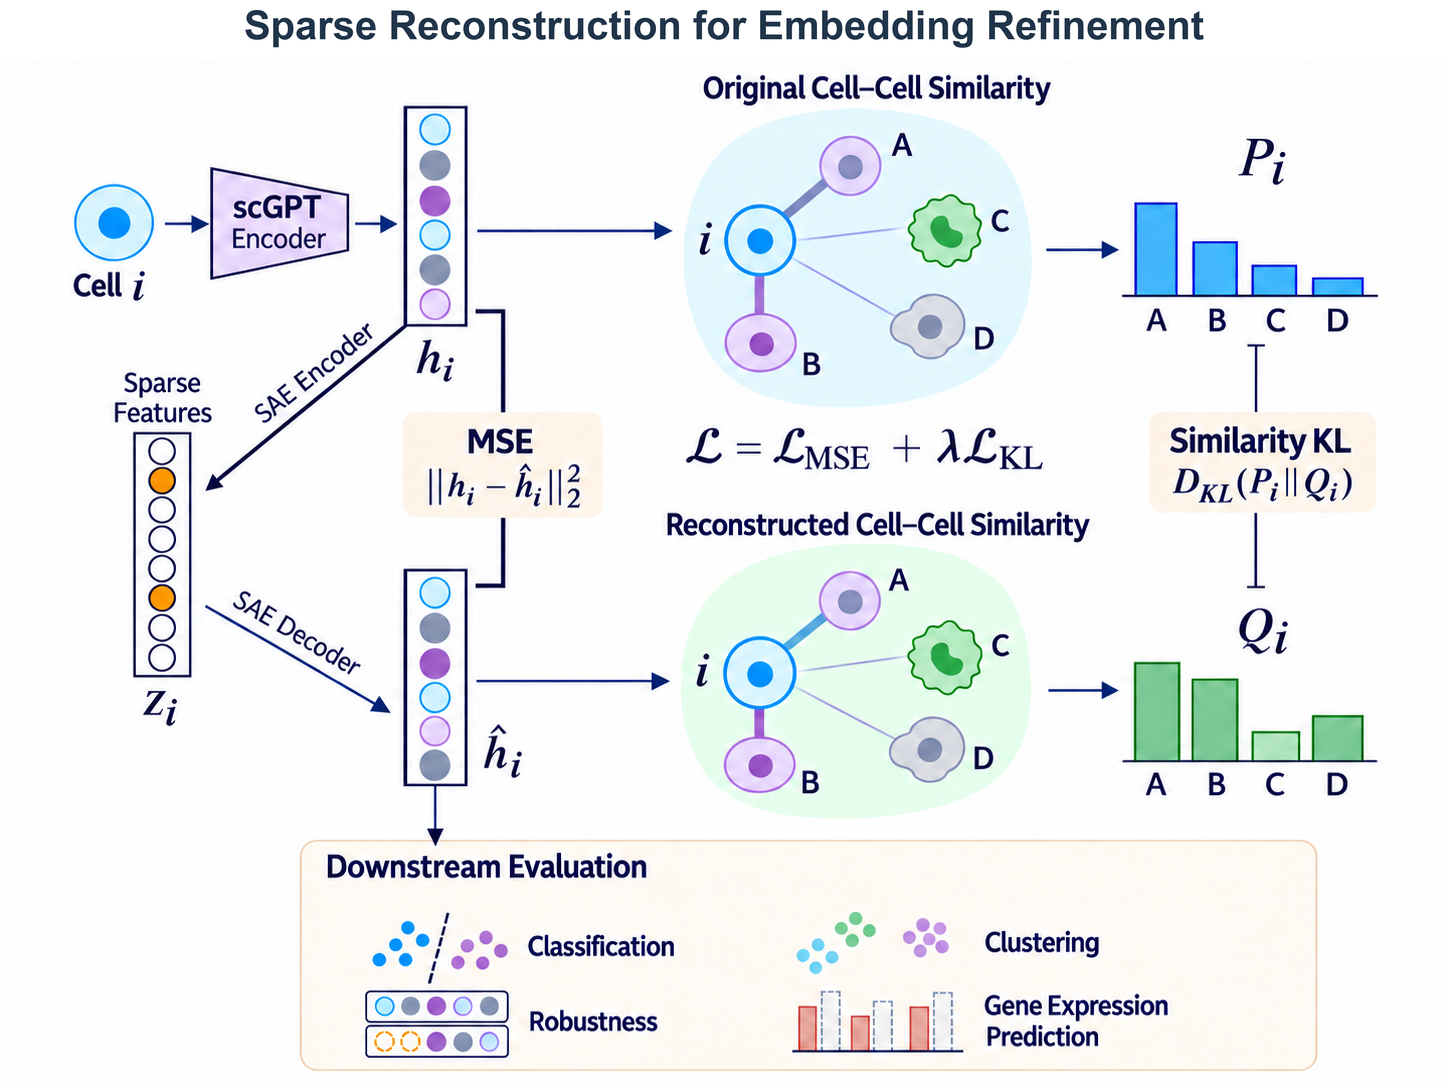
\includegraphics[width=0.90\linewidth]{images/figure1_model_overview.png}
  \caption{\textbf{Overview of structure-preserving sparse reconstruction for cell embedding refinement.} Cell embeddings extracted from a frozen scGPT encoder are decomposed and reconstructed using a Top-K sparse autoencoder (SAE). The training objective combines mean squared error (MSE) for point-wise reconstruction with KL divergence to encourage preservation of cell--cell similarity distributions. The reconstructed embeddings are subsequently evaluated for reconstruction fidelity, clustering, and downstream predictive performance, with additional analyses of robustness and gene expression prediction.}
  \label{fig:model-overview}
\end{figure}
\FloatBarrier

\section{Related Work}
\label{sec:related-work}

\subsection{Interpretability of Single-Cell Foundation Models}

Single-cell foundation models, such as Geneformer and scGPT, learn cellular representations that support diverse biological tasks. Existing interpretability approaches, including attention analysis and \textit{in silico} gene perturbation, provide insights into model behavior \citep{theodoris2023}. However, understanding how biological information is distributed across high-dimensional representations remains challenging, motivating feature-level interpretability methods.

\subsection{Sparse Autoencoders for Biological Interpretation}

Sparse autoencoders (SAEs) have been widely explored for extracting interpretable features from language models \citep{bricken2023}. Subsequent work introduced Top-K SAEs to improve the trade-off between sparsity and reconstruction fidelity \citep{gao2025}. More recently, \citet{claye2025} applied SAEs to single-cell models, combining sparse feature extraction with gene-level attribution and functional interpretation. \citet{pedrocchi2025} further demonstrated feature-level interventions for reducing technical variation, while \citet{kendiukhov2026} investigated cell-type-associated features and sparsity trade-offs. Building on these studies, we focus on the relationship between biological interpretability and the preservation of downstream representation utility.

\subsection{Structure-Preserving Representation Learning}

Conventional reconstruction objectives primarily minimize point-wise errors, which do not necessarily preserve relationships among samples. Relational learning methods, such as Relational Knowledge Distillation \citep{park2019}, have demonstrated the value of preserving inter-sample structure. Inspired by this principle, we investigate whether combining conventional reconstruction with KL-divergence-based alignment of cell--cell similarity distributions can better preserve the structure and downstream utility of scGPT embeddings.

\section{Methodology}
\label{sec:methodology}

\subsection{Problem Formulation and Sparse Representation}

Given a single-cell gene expression profile \(x_i\), we extract its embedding \(h_i \in \mathbb{R}^{d}\) using a pretrained, frozen scGPT encoder \(f_\theta\):

\[
h_i=f_\theta(x_i).
\]

We employ a Top-K sparse autoencoder (SAE) to decompose cell embeddings into sparse latent features. Let \(\mu\) denote the mean embedding computed from the training set. The encoding and reconstruction processes are defined as

\[
a_i=W_e(h_i-\mu)+b_e,
\]

\[
z_i=\operatorname{TopK}_{32}(a_i),
\qquad
\hat h_i=W_dz_i+\mu,
\]

where \(z_i\in\mathbb{R}^{m}\) is the sparse representation and \(\hat h_i\) is the reconstructed embedding. The Top-K operator retains the 32 largest activation values while preserving their signs. Decoder dictionary columns are constrained to unit norm after parameter updates.

We investigate two complementary applications of this framework: biological interpretation of sparse features and structure-preserving embedding reconstruction. The interpretation experiments use fixed baseline SAE checkpoints, whereas the refinement experiments evaluate checkpoints obtained through additional reconstruction-based optimization.

\subsection{Biological Interpretation of Sparse Features}

We investigate the biological relevance of learned sparse features through cell-type associations and gene-level attribution, as illustrated in Figure~\ref{fig:interpretability}.

\textbf{Cell-type association.} For each SAE feature, we quantify its ability to discriminate a target cell type from other cells using the area under the receiver operating characteristic curve (AUROC). Feature activations serve as discrimination scores, and cell-type annotations provide binary labels. We additionally evaluate feature discrimination on held-out donors.

\textbf{Gene-level attribution.} To examine how individual genes influence feature activation, we employ an input-substitution approach. Let \(s_j(x)\) denote the activation of SAE feature \(j\) for input \(x\):

\[
s_j(x)=z_j(f_\theta(x)).
\]

The contribution of gene \(g\) is estimated by replacing its expression-bin value with that of a reference cell \(r\):

\[
\Delta_{g,j}(i,r)
=
s_j(x_i)
-
s_j\left(x_i^{g\leftarrow r}\right).
\]

Here, \(x_i^{g\leftarrow r}\) differs from the original input only in the expression-bin value of gene \(g\), while other input values and gene tokens remain unchanged. Positive attribution indicates that substitution reduces feature activation, whereas negative attribution indicates an increase.

In our B-cell case study, reference cells are selected from the same donor and cell type, with zero activation of the target feature and proximity in the original embedding space. Attribution scores are aggregated across references, target cells, and donors. Genes with prominent positive contributions are subsequently examined using functional annotations to identify candidate biological associations.

\begin{figure}[!htbp]
  \centering
  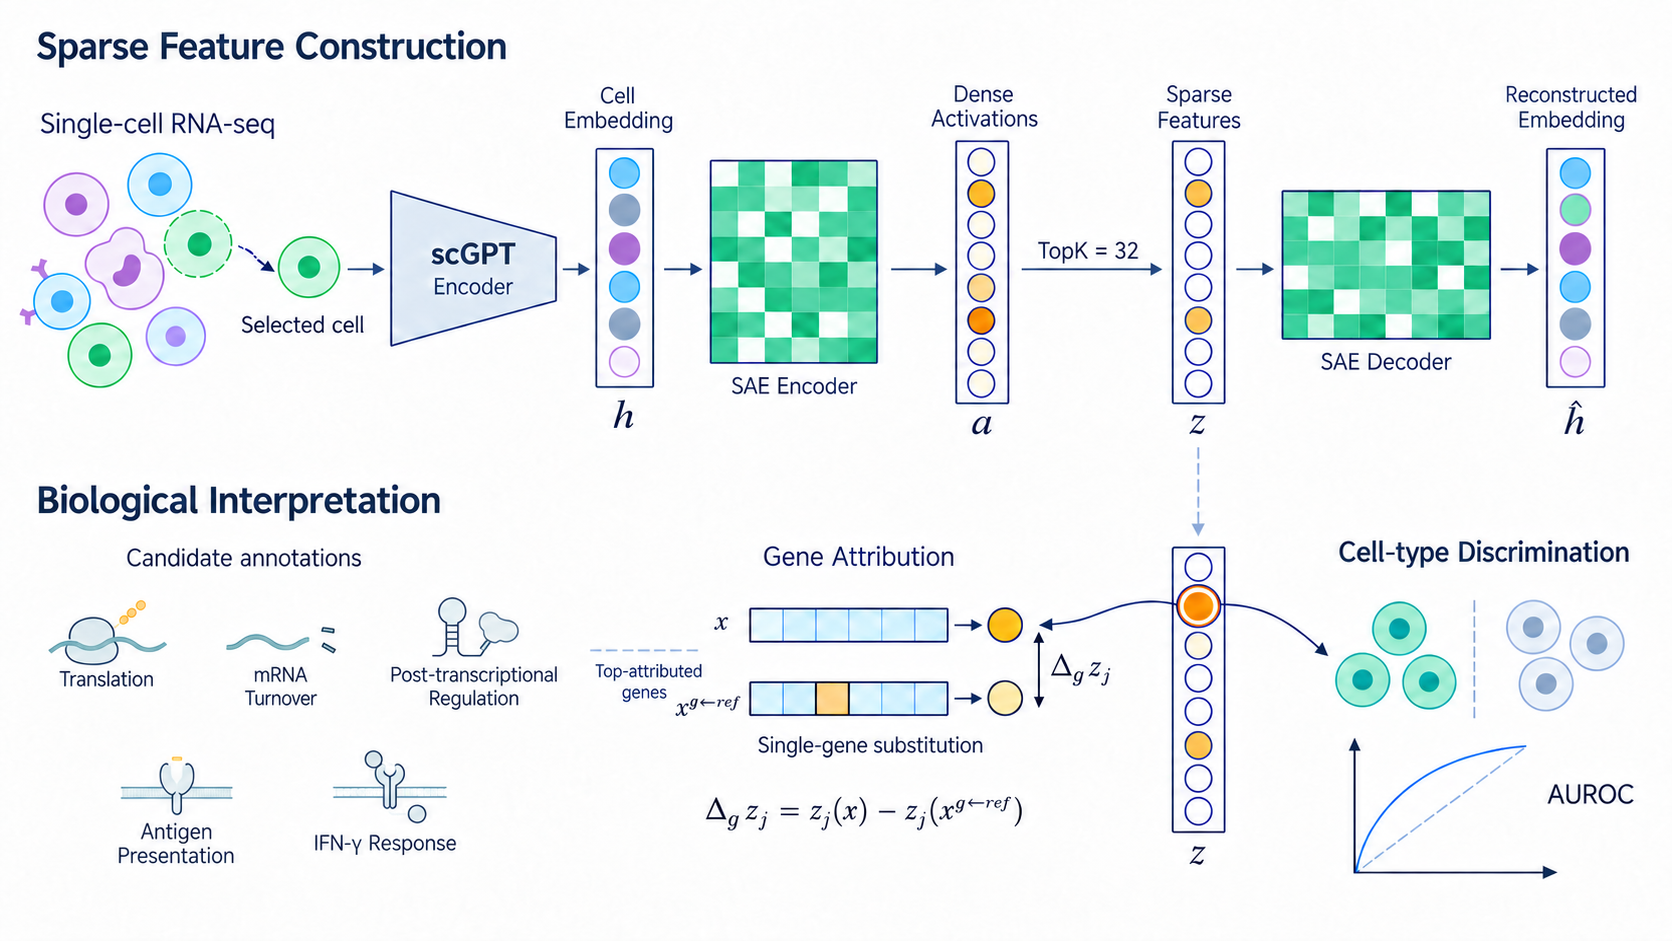
\includegraphics[width=\linewidth]{images/figure2_interpretability.png}
  \caption{\textbf{Sparse feature construction and biological interpretation.} Cell embeddings extracted from a frozen scGPT encoder are decomposed into sparse features using a Top-K SAE ($k=32$). The learned features are evaluated through cell-type discrimination (AUROC) and gene-input substitution attribution. Highly attributed genes are further examined to identify candidate biological functions associated with individual sparse features.}
  \label{fig:interpretability}
\end{figure}
\FloatBarrier

\subsection{Structure-Preserving Sparse Reconstruction}

Conventional SAE reconstruction minimizes the discrepancy between original and reconstructed embeddings. To account for the scale of the original representations, we normalize the reconstruction error by the training-set embedding variance:

\[
s_{\mathrm{train}}^2
=
\frac{1}{N_{\mathrm{train}}d}
\sum_{i\in\mathrm{Train}}
\|h_i-\mu\|_2^2,
\]

\[
\mathcal L_{\mathrm{MSE}}
=
\frac{1}{Bd\,s_{\mathrm{train}}^2}
\sum_{i\in\mathcal B}
\|h_i-\hat h_i\|_2^2,
\]

where \(\mathcal B\) denotes a minibatch of \(B\) cells.

Although MSE encourages accurate reconstruction of individual embeddings, it does not explicitly preserve the similarity relationships among cells. We therefore introduce a relational regularizer based on Kullback--Leibler (KL) divergence.

First, we compute mean-centered, normalized embeddings:

\[
u_i=\frac{h_i-\mu}
{\max(\|h_i-\mu\|_2,\epsilon)},
\qquad
v_i=\frac{\hat h_i-\mu}
{\max(\|\hat h_i-\mu\|_2,\epsilon)}.
\]

For each cell \(i\), we define similarity distributions over an allowed comparison set \(\mathcal A_i\) within the current minibatch:

\[
P_{ij}
=
\frac{\exp(u_i^\top u_j/\tau)}
{\sum_{k\in\mathcal A_i}\exp(u_i^\top u_k/\tau)},
\]

\[
Q_{ij}
=
\frac{\exp(v_i^\top v_j/\tau)}
{\sum_{k\in\mathcal A_i}\exp(v_i^\top v_k/\tau)},
\]

where \(\tau=0.1\) is the temperature parameter. The allowed comparison set excludes self-comparisons and may impose additional dataset-specific donor restrictions.

We minimize the divergence between the original and reconstructed similarity distributions:

\[
\mathcal L_{\mathrm{KL}}
=
\frac{1}{B}
\sum_{i\in\mathcal B}
\sum_{j\in\mathcal A_i}
P_{ij}\log\frac{P_{ij}}{Q_{ij}}.
\]

The original similarity distribution \(P\) is treated as a fixed target, while gradients propagate through the reconstructed embeddings used to construct \(Q\).

The overall objective is

\[
\boxed{
\mathcal L_{\mathrm{total}}
=
\mathcal L_{\mathrm{MSE}}
+
\lambda\mathcal L_{\mathrm{KL}}
}
\]

where \(\lambda\) controls the strength of relational regularization.

By combining point-wise reconstruction with relational alignment, our objective seeks to preserve both individual cell representations and their relative similarity structure. We assess its effectiveness through reconstruction fidelity, clustering performance, and robustness under different evaluation conditions.

\section{Experiments}
\label{sec:experiments}

\subsection{Experimental Setup}

We evaluate our framework on three single-cell datasets: Kang control, Kang interferon-stimulated, and PBMC. Cell embeddings are extracted using a frozen scGPT encoder and decomposed using Top-K SAEs with $k=32$. Biological interpretability is evaluated through cell-type discrimination and gene-input attribution. For embedding refinement, we compare original scGPT embeddings, MSE-based SAE reconstruction, and relationally regularized reconstruction (MSE + KL). Downstream performance is assessed through classification, clustering, expression prediction, and robustness evaluations, with the latter two conducted using a separate expression-supervised SAE extension.

The Kang data originate from the control and interferon-$\beta$ stimulation experiment in \href{https://www.ncbi.nlm.nih.gov/geo/query/acc.cgi?acc=GSE96583}{GEO accession GSE96583}. Our analysis includes 9,577 control and 9,728 stimulated cells from the same six donors. Each condition is evaluated separately in six donor-held-out folds, with four donors for training, one for validation, and one for testing. The additional PBMC collection, supplied as \texttt{PBMC368k\_raw.h5ad}, contributes 4,638 cells from two annotated batches (\texttt{Batch1\_3k} and \texttt{Batch2\_68k\_r}). We evaluate both source-to-target batch directions, reserving approximately 20\% of source-batch cells for class-stratified validation and the entire other batch for testing. These batch labels are not treated as verified donor identities.

For each dataset and split, a $512\!\rightarrow\!2048\!\rightarrow\!512$ SAE is fitted to training embeddings. Classification uses a class-balanced linear Ridge readout on representations standardized using training-set statistics; its regularization strength is selected by validation Macro-F1, and test Macro-F1 is computed over the fixed set of eight cell types. Clustering is performed independently within each held-out test group using Leiden clustering on a cosine 15-nearest-neighbor graph, after centering representations by the original training-embedding mean. We use the RBConfiguration objective with resolution 1.0 and assess agreement with cell-type annotations using adjusted Rand index (ARI), without selecting the resolution using test labels.

\subsection{Biological Interpretability}

\textbf{Cell-type-associated features.} Figure~\ref{fig:celltype} illustrates the activation patterns of selected SAE features across major cell types. Several features exhibit cell-type-specific activation and achieve high discrimination AUROC across donors, particularly for B cells and monocytes. These results suggest that sparse representations capture identifiable cellular information.

\begin{figure}[!htbp]
  \centering
  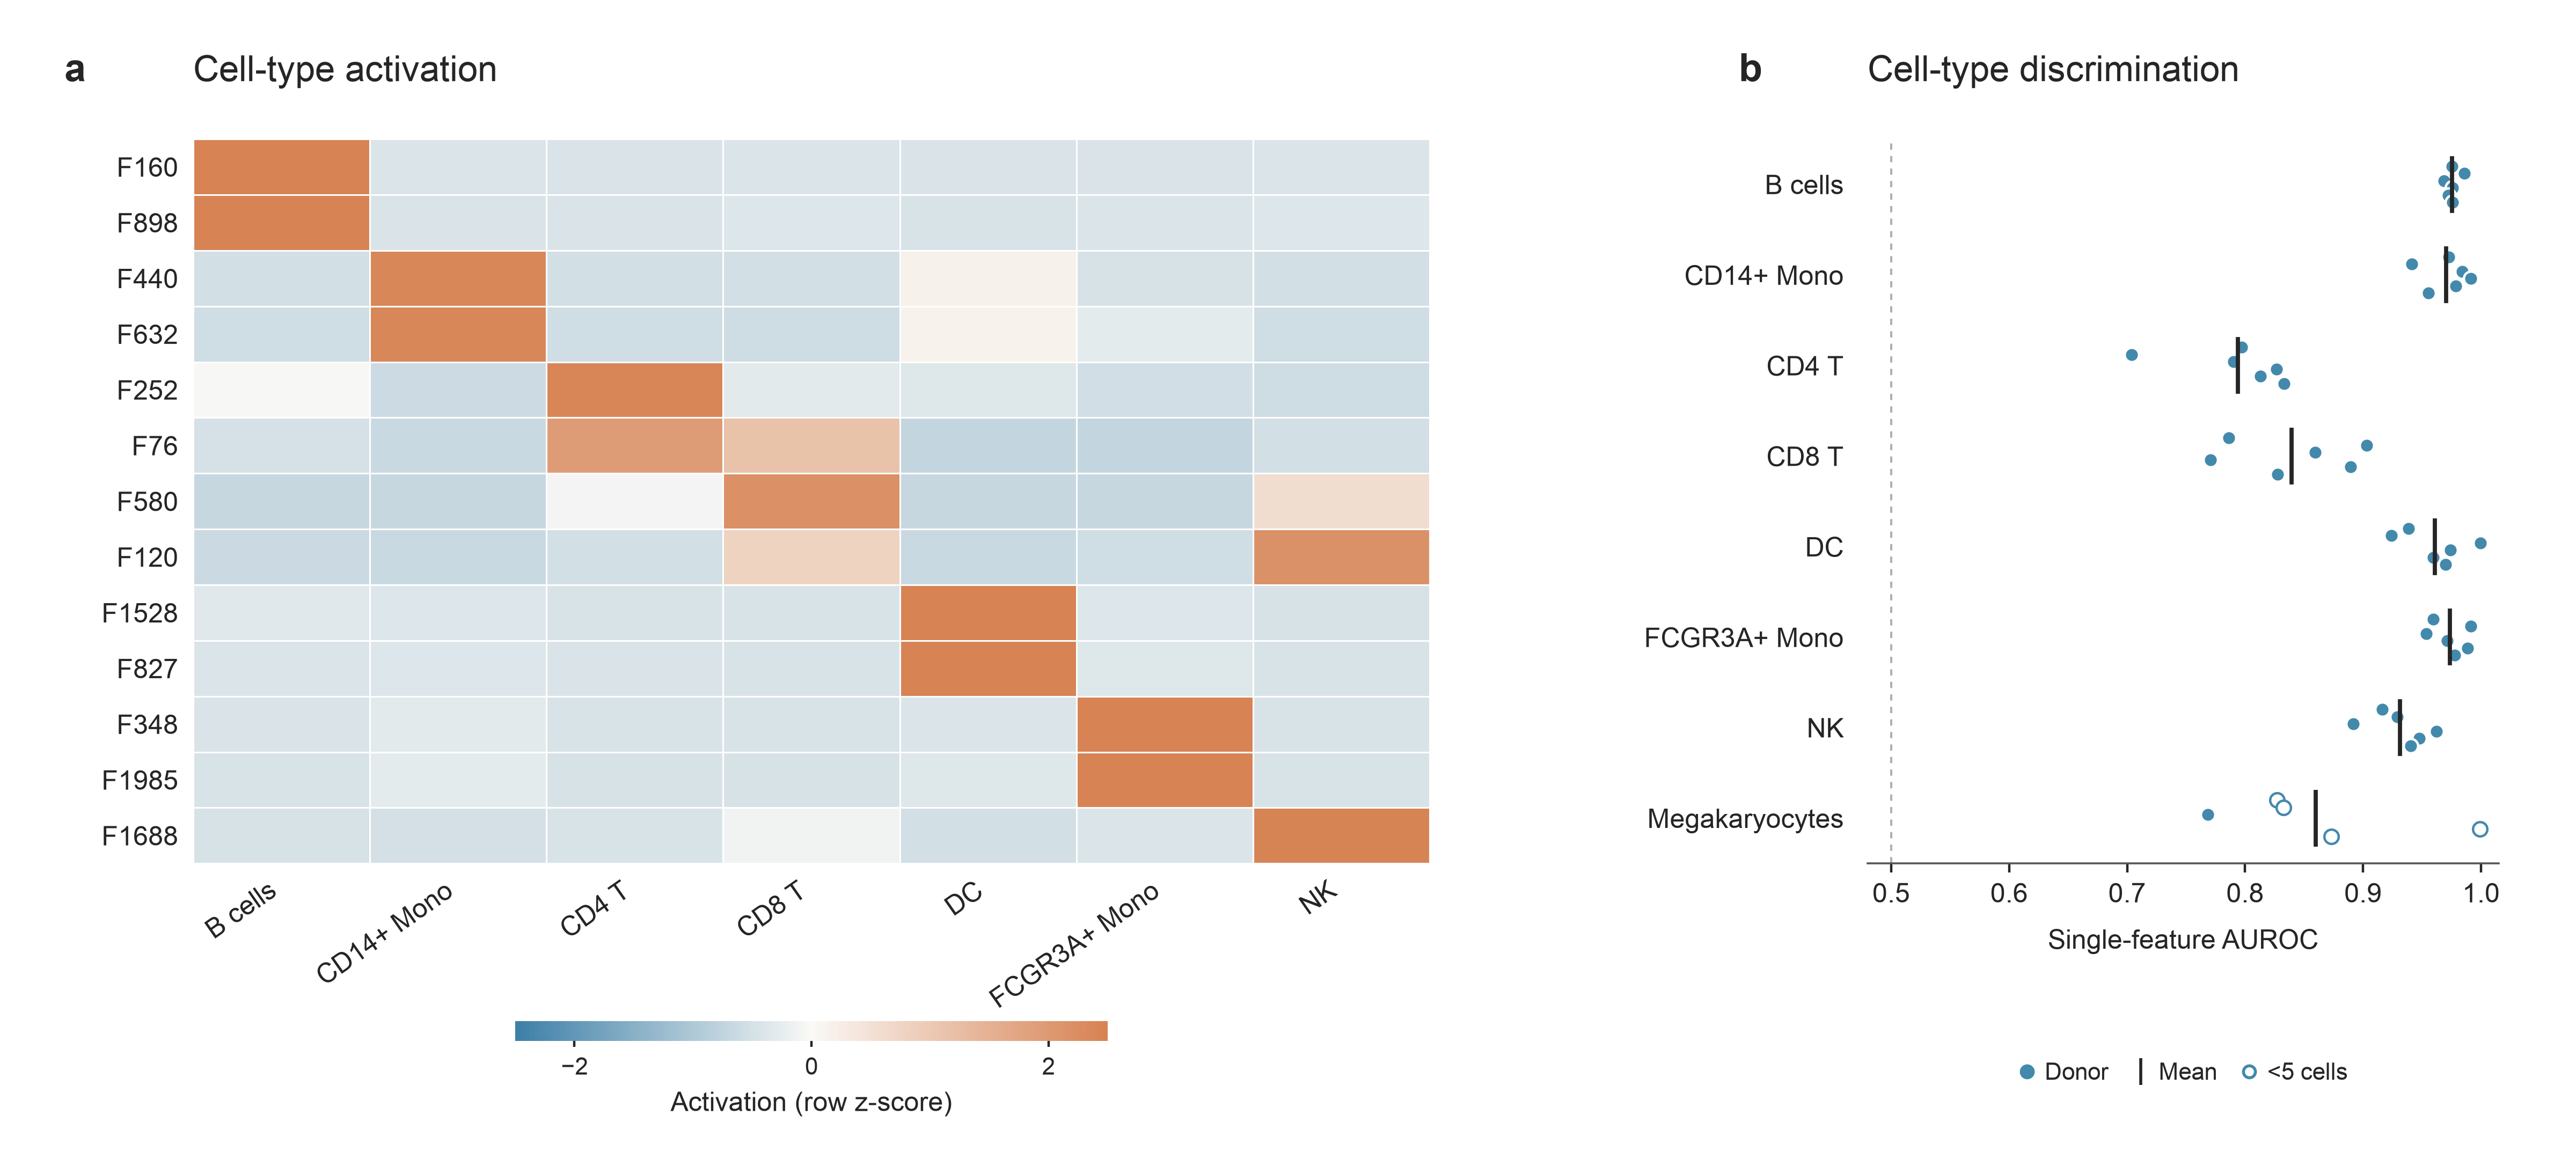
\includegraphics[width=\linewidth]{images/figure3_celltype.png}
  \caption{\textbf{Cell-type-associated sparse features in scGPT representations.} Activation patterns of selected SAE features across major cell types and their cell-type discrimination performance, measured by AUROC on held-out donors. The results illustrate the specificity and variability of sparse feature associations with cellular identities.}
  \label{fig:celltype}
\end{figure}

\textbf{Gene-level interpretation.} We further investigate the B-cell-associated feature F160 (Figure~\ref{fig:f160}). F160 exhibits strong activation in B cells but remains largely inactive in other cell types. Attribution-guided gene substitution produces larger activation reductions than matched random substitution, supporting the relevance of the identified gene contributions. Functional analysis reveals associations with ribosomal proteins, RNA-related processes, and antigen presentation, providing candidate biological interpretations of this feature.

\begin{figure}[!htbp]
  \centering
  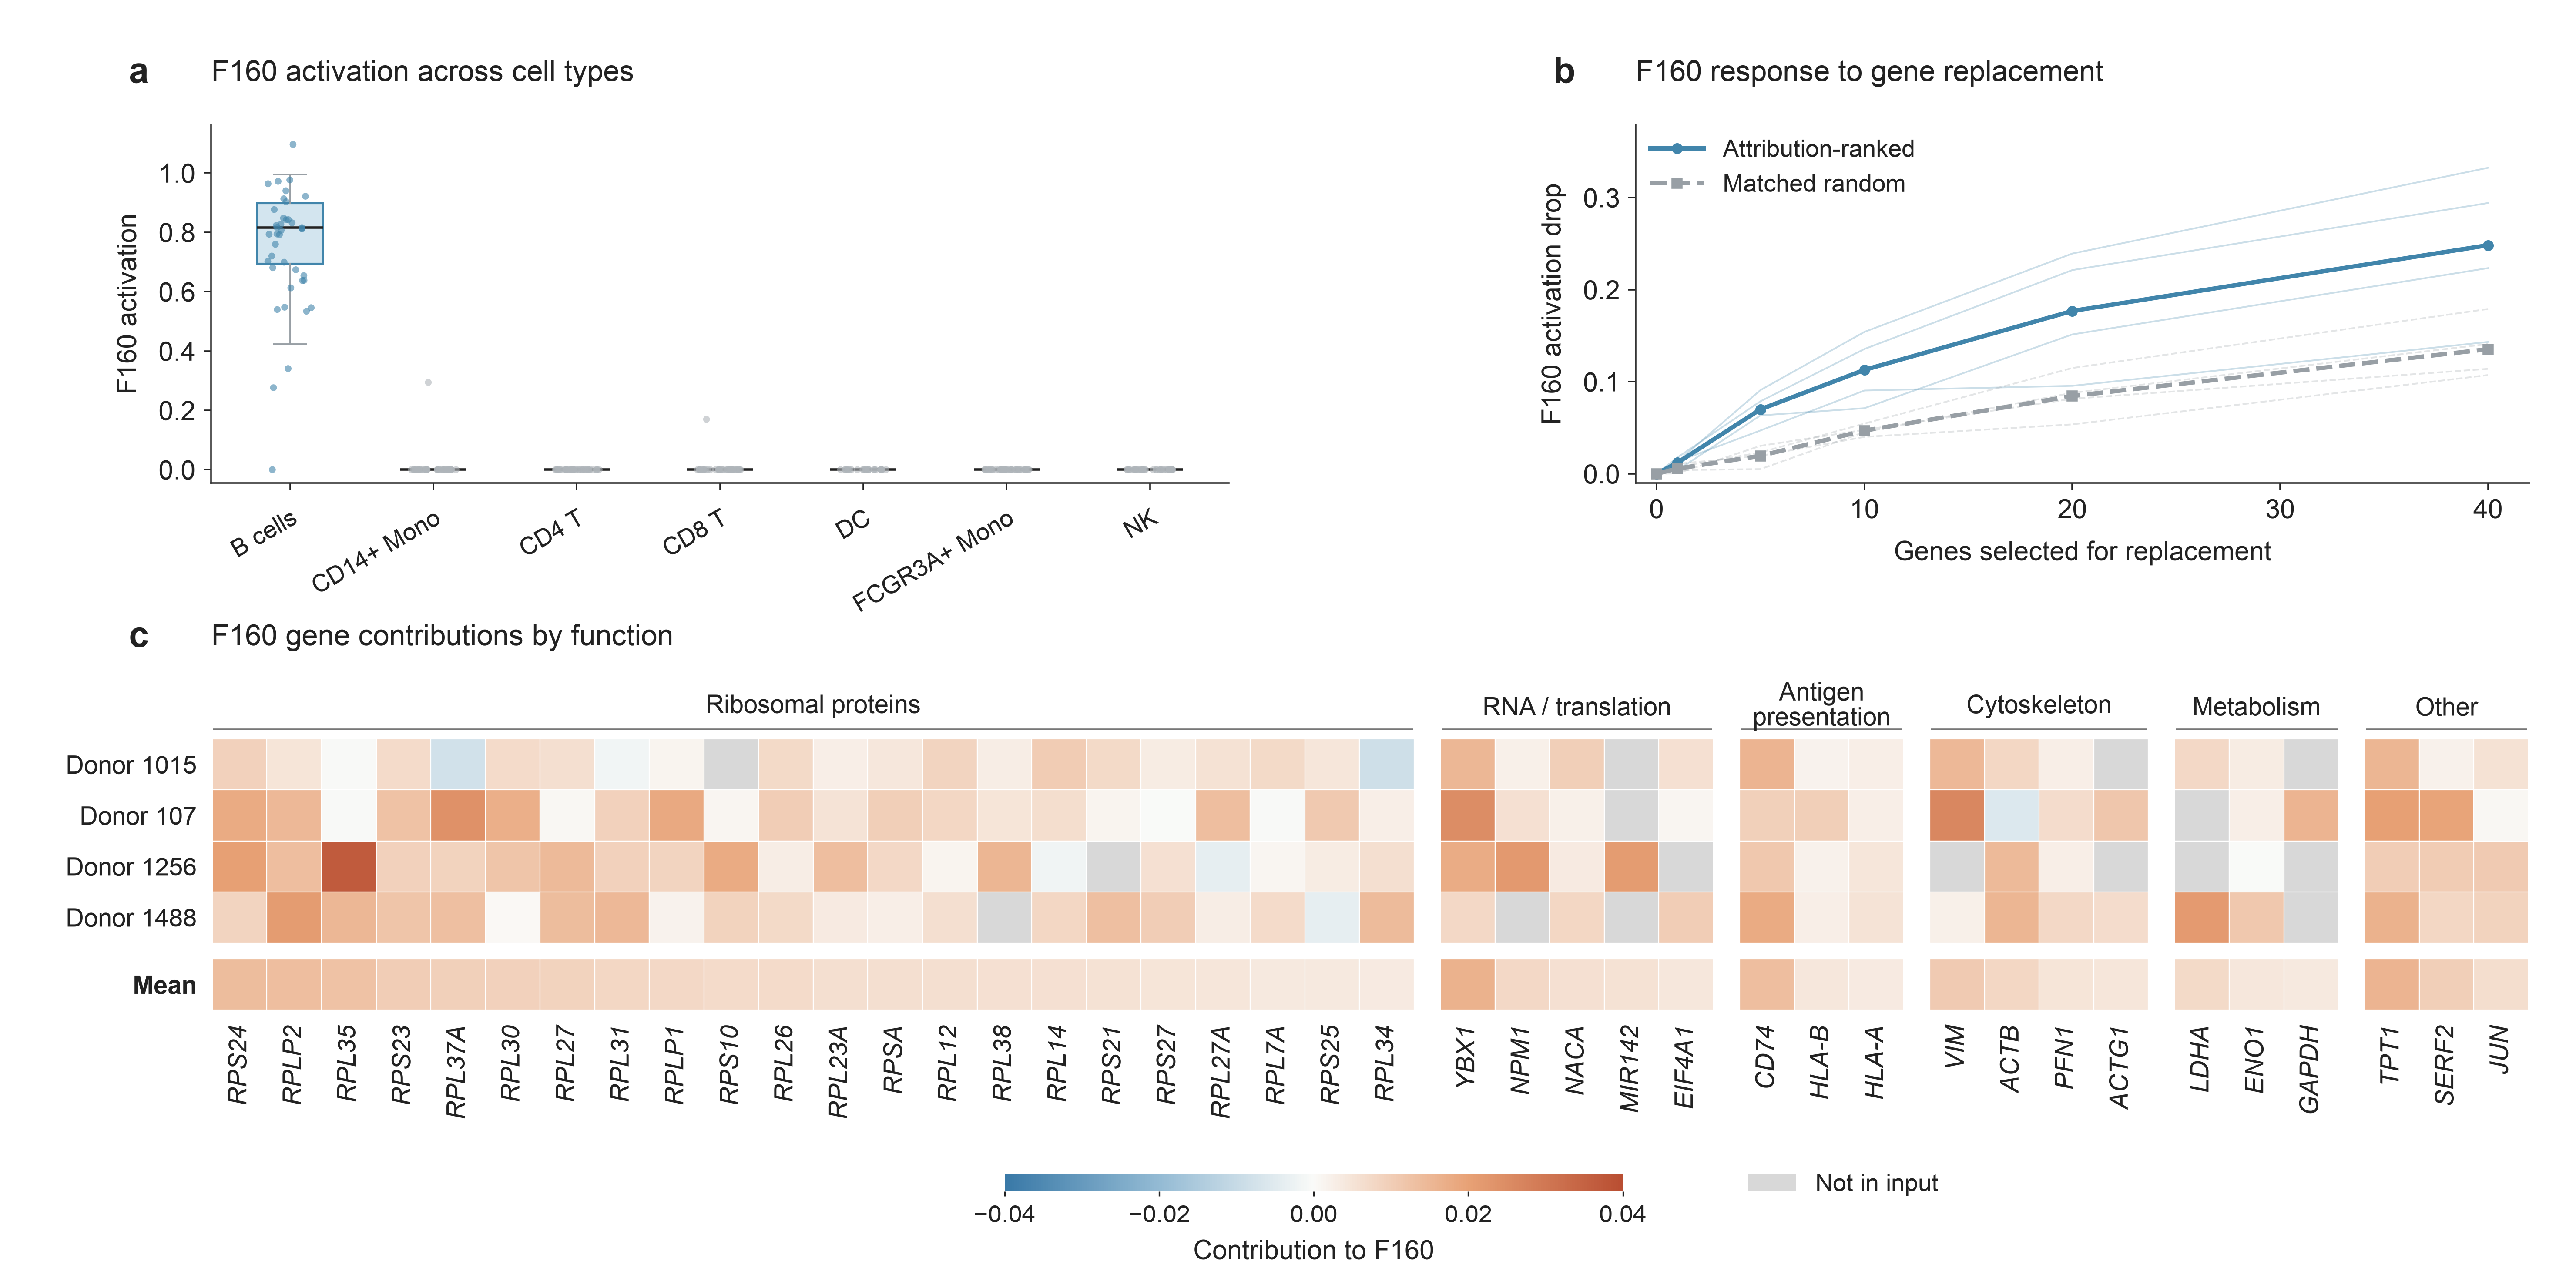
\includegraphics[width=\linewidth]{images/figure4_f160.png}
  \caption{\textbf{Biological interpretation of the B-cell-associated feature F160.} (a) Feature activation across cell types. (b) Changes in F160 activation following attribution-guided gene-input substitution compared with matched random substitution. (c) Gene-level attribution patterns and candidate functional associations, including ribosomal processes and antigen presentation.}
  \label{fig:f160}
\end{figure}

\FloatBarrier
\subsection{Embedding Refinement and Downstream Evaluation}

\textbf{Classification performance.} Table~\ref{tab:classification} presents the Macro-F1 scores of different representations. With the best observed KL weights, SAE reconstruction achieves improvements of 1.42, 0.73, and 0.67 percentage points over the original embeddings on Kang control, Kang stimulated, and PBMC, respectively. However, these improvements are not consistent under a fixed regularization weight.

\begin{table}[!htbp]
  \caption{\textbf{Cell-type classification performance of original and SAE-reconstructed embeddings.} Macro-F1 scores (\%) are reported for original scGPT embeddings, MSE-only SAE reconstruction, and MSE + KL reconstruction across three datasets. The best observed KL weights are reported for each dataset.}
  \label{tab:classification}
  \centering
  \small
  \setlength{\tabcolsep}{5pt}
  \renewcommand{\arraystretch}{1.15}
  \begin{tabular*}{\linewidth}{@{\extracolsep{\fill}}lrrr@{}}
    \toprule
    Representation & Kang ctrl & Kang stim & PBMC \\
    \midrule
    Original embedding & 82.75 & 84.52 & 82.68 \\
    SAE: MSE & 83.01 & 84.19 & 81.79 \\
    SAE: MSE + KL ($\lambda=0.3$) & \textbf{84.18} & 83.62 & 81.61 \\
    SAE: MSE + KL (best $\lambda$) & \textbf{84.18} & \textbf{85.26} & \textbf{83.34} \\
    \midrule
    $\Delta$ vs. original (best $\lambda$) & $+1.42$ & $+0.73$ & $+0.67$ \\
    \bottomrule
  \end{tabular*}
  \par\vspace{3pt}
  \begin{minipage}{\linewidth}
    \footnotesize
    Best observed KL weights were selected retrospectively using test performance. Bold indicates the best value in each column; $\Delta$ is measured in percentage points.
  \end{minipage}
\end{table}


\textbf{Additional downstream evaluations.} Figure~\ref{fig:downstream} evaluates expression prediction, input-masking robustness, and clustering. The separate expression-supervised SAE reduces masked-gene prediction error across the evaluated datasets and improves masking robustness on Kang data, while performance deteriorates on PBMC. For clustering, SAE-reconstructed embeddings generally exhibit lower ARI than the original representations, and KL regularization does not consistently outperform MSE-only reconstruction.

\begin{figure}[!htbp]
  \centering
  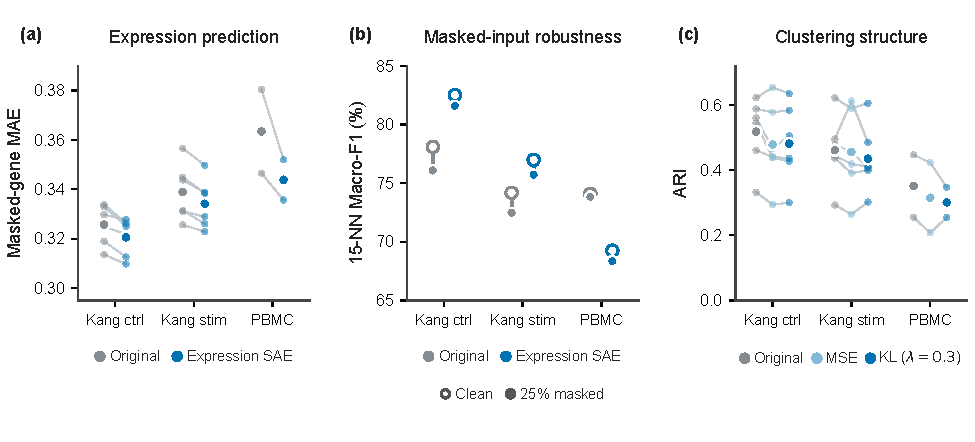
\includegraphics[width=\linewidth]{images/figure5_downstream.pdf}
  \caption{\textbf{Downstream evaluation of SAE-based representations.} (a) Masked-gene expression prediction error using a separately trained expression-supervised SAE. (b) Classification robustness under input masking across datasets. (c) Clustering performance measured by adjusted Rand index (ARI) for original and reconstructed embeddings. Expression prediction and masking robustness are evaluated separately from the MSE + KL reconstruction objective.}
  \label{fig:downstream}
\end{figure}

\textbf{Sensitivity to relational regularization.} Figure~\ref{fig:sensitivity} examines the effect of the KL weight $\lambda$ across the three datasets. The best observed performance occurs at $\lambda=0.3$ for Kang control and $\lambda=0.03$ for both Kang stimulated and PBMC. Performance varies non-monotonically with $\lambda$, indicating that the effectiveness of relational regularization depends on the dataset and hyperparameter configuration.

\begin{figure}[!htbp]
  \centering
  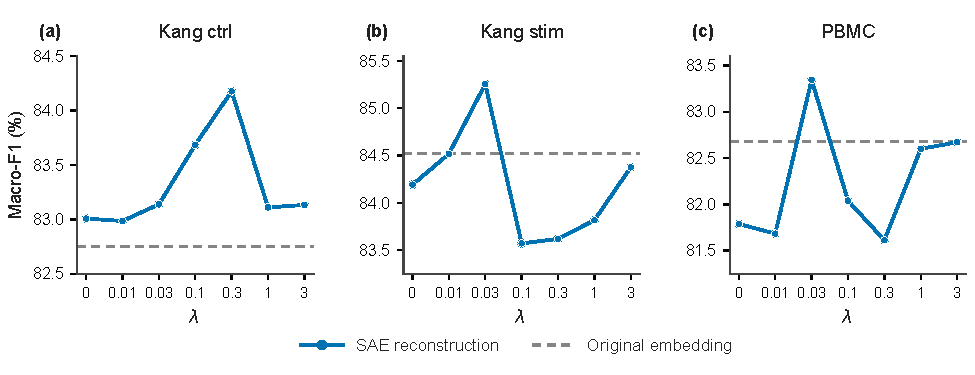
\includegraphics[width=\linewidth]{images/figure6_sensitivity.pdf}
  \caption{\textbf{Sensitivity to the relational regularization weight.} Cell-type classification performance (Macro-F1) across different KL weights ($\lambda$) on (a) Kang control, (b) Kang stimulated, and (c) PBMC datasets. The results illustrate dataset-dependent sensitivity to relational regularization. Dashed horizontal lines indicate the performance of the original scGPT embeddings.}
  \label{fig:sensitivity}
\end{figure}

\FloatBarrier

Overall, these results indicate that SAE-based reconstruction can improve selected downstream outcomes, but its benefits remain task- and dataset-dependent. Biological interpretability, reconstruction fidelity, and downstream utility therefore require complementary evaluation.

\section{Discussion}
\label{sec:discussion}

Our results highlight both the potential and limitations of SAE-based interpretation and refinement of single-cell representations. Sparse features exhibit strong cell-type associations, while gene-input attribution provides insights into the biological information encoded by scGPT. These findings are consistent with prior SAE-based analyses of single-cell foundation models \citep{claye2025,pedrocchi2025}. However, these associations reflect model-level responses rather than direct evidence of biological causality.

From a representation learning perspective, our experiments reveal that reconstruction fidelity and downstream utility do not necessarily improve together. Although relational regularization improves classification in selected settings, its benefits depend on the dataset and regularization strength, and clustering performance is not consistently preserved. This observation is consistent with broader SAE evaluations in language models, where improvements in proxy metrics do not reliably translate into gains in practical utility \citep{karvonen2025}. These observations suggest that maintaining cell--cell similarity alone may be insufficient to retain all task-relevant information.

Our study has several limitations. The experiments primarily focus on scGPT and PBMC datasets, limiting conclusions about broader generalization. Independent zero-shot evaluations of single-cell foundation models likewise highlight the need to assess representation quality across datasets and tasks \citep{kedzierska2025}. Moreover, the biological interpretations require further validation using independent data and experimental perturbations. A more comprehensive evaluation of structural preservation and hyperparameter stability is also needed to establish when relational regularization provides reliable benefits.

\section{Conclusion and Future Work}
\label{sec:conclusion}

We investigated sparse autoencoders for interpreting and refining scGPT cell representations. Our findings show that SAE features capture cell-type-associated signals and provide candidate biological interpretations through gene-level attribution. We further explored structure-preserving reconstruction using MSE and KL divergence, demonstrating potential improvements in selected downstream settings while revealing task-dependent performance trade-offs.

Future work will focus on two directions. First, we aim to evaluate the generalizability of our framework across different single-cell foundation models, including Geneformer \citep{theodoris2023} and scFoundation \citep{hao2024}. Second, we plan to investigate more expressive autoencoder architectures, such as hierarchical SAEs \citep{bussmann2025} and subspace-aware SAEs \citep{dalili2026}, to explore whether cellular representations can be decomposed into biologically meaningful latent subspaces associated with cell identity, functional states, and regulatory programs.

\bibliographystyle{plainnat}
\bibliography{references}

\end{document}
